\let\lesson\undefined
\newcommand{\lesson}{\phantomlesson{Bài 2.}}


\setcounter{section}{2}
\section{Bài tập trắc nghiệm}
\begin{enumerate}[label=\bfseries Câu \arabic*:, leftmargin=1.7cm]
	\item \mkstar{1}\\
	Khi nhiệt độ của vật tăng lên thì
	\begin{mcq}
		\item động năng của các phân tử cấu tạo nên vật tăng.
		\item động năng của các phân tử cấu tạo nên vật giảm.
		\item nội năng của vật tăng.
		\item thế năng của các phân tử cấu tạo nên vật tăng.
	\end{mcq}
\hideall{
\textbf{Đáp án A.}
}

\item \mkstar{1}\\
Nội năng của một hệ là 
\begin{mcq}
	\item tổng động năng chuyển động nhiệt và thế năng tương tác giữa các phân tử cấu tạo nên hệ.
	\item tổng của động năng và thế năng của hệ.
	\item tổng động năng chuyển động của các phân tử cấu tạo nên hệ.
	\item tổng động lượng chuyển động hỗn loạn và thế năng tương tác giữa các phân tử cấu tạo nên hệ.
\end{mcq}
\hideall{
\textbf{Đáp án A.}
}

\item \mkstar{1}\\
Nội năng của một hệ phụ thuộc vào
\begin{mcq}(2)
	\item nhiệt độ của hệ.
	\item thể tích của hệ.
	\item nhiệt độ và thể tích của hệ.
	\item nhiệt độ, thể tích và khối lượng của hệ.
\end{mcq}
\hideall{
\textbf{Đáp án C.}
}

\item \mkstar{1}\\
Cách làm thay đổi nội năng của hệ bằng hình thức thực hiện công là
\begin{mcq}
	\item bỏ thỏi sắt vào nước nóng.
	\item chà sát miếng kim loại bằng giấy nhám.
	\item đưa một thỏi sắt lên cao.
	\item hơ thỏi sắt bằng đèn cồn.
\end{mcq}
\hideall{
\textbf{Đáp án B.}
}

\item \mkstar{1}\\
Khi ấn piston để nén khí trong một cylanh thì
\begin{mcq}(2)
	\item kích thước mỗi phân tử khí giảm.
	\item khoảng cách giữa các phân tử khí giảm.
	\item khối lượng mỗi phân tử khí giảm.
	\item số phân tử khí giảm.
\end{mcq}
\hideall{
\textbf{Đáp án B.}
}
\item \mkstar{1}\\
Định luật I của nhiệt động lực học là vận dụng định luật nào sau đây?
\begin{mcq}
	\item Định luật bảo toàn động lượng.
	\item Định luật bảo toàn cơ năng.
	\item Định luật bảo toàn và chuyển hoá năng lượng.
	\item Các định luật Newton về chuyển động.
\end{mcq}
\hideall{
\textbf{Đáp án C.}
}

\item \mkstar{1}\\
Khi nói về nội dung của định luật I nhiệt động lực học, phát biểu nào sau đây là \textbf{sai}?
\begin{mcq}
	\item Vật nhận nhiệt, nội năng của vật tăng.
	\item Vật truyền nhiệt, nội năng của vật giảm.
	\item Độ biến thiên nội năng của vật bằng tổng công và nhiệt lượng mà vật nhận được.
	\item Độ biến thiên nội năng của vật bằng hiệu giữa công và nhiệt lượng mà vật nhận được.
\end{mcq}
\hideall{
\textbf{Đáp án D.}
}

\item \mkstar{1}\\
Hệ thức $\Delta U=Q+A$ khi $Q>0$ và $A<0$ mô tả quá trình
\begin{mcq}(2)
	\item hệ truyền nhiệt và sinh công.
	\item hệ nhận nhiệt và sinh công.
	\item hệ truyền nhiệt và nhận công.
	\item hệ nhận nhiệt và nhận công.
\end{mcq}
\hideall{
\textbf{Đáp án B.}
}

\item \mkstar{1}\\
Dùng tay nén piston và đồng thời nung nóng khối khí trong cylanh. Xác định dấu của $Q$ và $A$ của khối khí trong biểu thức của định luật I nhiệt động lực học $\Delta U=Q+A$.
\begin{mcq}(4)
	\item $A>0$; $Q>0$.
	\item $A<0$; $Q>0$.
	\item $A>0$; $Q<0$.
	\item $A<0$; $Q<0$.
\end{mcq}
\hideall{
\textbf{Đáp án A.}
}

\item \mkstar{1}\\
Chọn phát biểu \textbf{đúng nhất}.
\begin{mcq}
	\item Động cơ nhiệt là động cơ trong đó toàn bộ phần năng lượng của nhiên liệu bị đốt cháy chuyển hoá thành cơ năng.
	\item Động cơ nhiệt là động cơ trong đó một phần năng lượng của nhiên liệu bị đốt cháy chuyển hoá thành nhiệt năng.
	\item Động cơ nhiệt là động cơ trong đó một phần năng lượng của nhiên liệu bị đốt cháy chuyển hoá thành cơ năng.
	\item Động cơ nhiệt là động cơ trong đó toàn bộ năng lượng của nhiên liệu bị đốt cháy chuyển hoá thành nhiệt năng.
\end{mcq}
\hideall{
\textbf{Đáp án C.}
}



\item \mkstar{2}\\
Khi thả một thỏi kim loại đã được nung nóng vào một chậu nước lạnh thì nội năng của thỏi kim loại và của nước thay đổi như thế nào?
\begin{mcq}
	\item Nội năng của thỏi kim loại và của nước đều tăng.
	\item Nội năng của thỏi kim loại và của nước đều giảm.
	\item Nội năng của thỏi kim loại giảm, nội năng của nước tăng.
	\item Nội năng của thỏi kim loại tăng, nội năng của nước giảm.
\end{mcq}
\hideall{
\textbf{Đáp án C.}
}

\item \mkstar{2}\\
Khi ôtô đóng kín cửa để ngoài trời nắng nóng, nhiệt độ không khí trong xe tăng rất cao so với nhiệt độ bên ngoài, làm giảm tuổi thọ các thiết bị trong xe. Nguyên nhân gây ra sự tăng nhiệt độ này là do thể tích khối khí trong ôtô
\begin{mcq}
	\item  thay đổi nên nhiệt lượng mà khối khí trong ôtô nhận được chủ yếu làm tăng nội năng của khối khí.
	\item không đổi nên nhiệt lượng mà khối khí trong ôtô nhận được chủ yếu làm giảm nội năng của khối khí.
	\item thay đổi nên nhiệt lượng mà khối khí trong ôtô nhận được chủ yếu làm tăng nội giảm của khối khí.
	\item không đổi nên nhiệt lượng mà khối khí trong ôtô nhận được chủ yếu làm tăng nội năng của khối khí.
\end{mcq}
\hideall{
\textbf{Đáp án D.}
}


\item \mkstar{3}\\
Người ta thực hiện công $\SI{100}{\joule}$ để nén khí trong một cylanh. Biết trong quá trình nén, khí truyền ra ngoài môi trường nhiệt lượng $\SI{20}{\joule}$. Độ biến thiên nội năng của khí là 
\begin{mcq}(4)
	\item $\SI{80}{\joule}$.
	\item $\SI{-80}{\joule}$.
	\item $\SI{120}{\joule}$.
	\item $\SI{60}{\joule}$.
\end{mcq}
\hideall{
\textbf{Đáp án A.}\\
Khí nhận công nên $A>0\Rightarrow A=\SI{100}{\joule}$, khí toả nhiệt ra ngoài nên $Q<0\Rightarrow Q=\SI{-20}{\joule}$.\\
Độ biến thiên nội năng của khí:
$$\Delta U=Q+A=\SI{80}{\joule}.$$
}

\item Khi truyền nhiệt lượng $\SI{6E6}{\joule}$ cho khí trong một cylanh hình trụ thì khí nở ra đẩy piston lên làm thể tích của khí tăng thêm $\SI{0.50}{\meter^3}$. Biết áp suất của khí là $\SI{8E6}{\newton/\meter^2}$ và coi áp suất này không đổi trong quá trình khí thực hiện công. Độ biến thiên nội năng của khí là
\begin{mcq}(4)
	\item $\SI{3E6}{\joule}$.
	\item $\SI{1.5E6}{\joule}$.
	\item $\SI{2E6}{\joule}$.
	\item $\SI{3.5E6}{\joule}$.
\end{mcq}
\hideall{
\textbf{Đáp án C.}\\
Công do khí thực hiện:
$$A'=F\Delta x=pS\Delta x=p\Delta V=\SI{4E6}{\joule}.$$
Vì khí thực hiện công nên $A<0\Rightarrow A=-A'=-\SI{4E6}{\joule}$.\\
Độ biến thiên nội năng của khí:
$$\Delta U=Q+A=\SI{2E6}{\joule}.$$
}

\item \mkstar{3}\\
Một khối khí chứa trong một cylanh đặt thẳng đứng, miệng cylanh được đậy kín bằng một piston nhẹ có tiết diện $\SI{10}{\centi\meter^2}$, có thể dịch chuyển không ma sát trong cylanh. Người ta kéo đều piston lên cao một đoạn $\SI{10}{\centi\meter}$. Biết nhiệt độ khối khí không đổi, áp suất khí quyển bằng $\SI{101325}{\pascal}$ và công do khối khí sinh ra trong quá trình này là $\SI{7.5}{\joule}$. Công cần thực hiện để kéo piston là
\begin{mcq}(4)
	\item $\SI{2.31}{\joule}$.
	\item $\SI{2.63}{\joule}$.
	\item $\SI{17.63}{\joule}$.
	\item $\SI{7.5}{\joule}$.
\end{mcq}
\hideall{
\textbf{Đáp án B.}\\
\begin{center}
	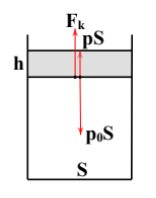
\includegraphics[width=0.25\linewidth]{../figs/VN12-Y24-PH-SYL-003P-2}
\end{center}
Piston được nâng lên đều nên:
$$F_k=\left(p_0-p\right)S.$$
Công cần thực hiện:
$$A=F_k\Delta h=\left(p_0-p\right)S\Delta h=p_0S\Delta h-A_\text{khí}=\SI{2.6325}{\joule}.$$
}

\end{enumerate}
\section{Trắc nghiệm đúng/sai}
\begin{enumerate}[label=\bfseries Câu \arabic*:, leftmargin=1.7cm]
	\item\mkstar{2}\\
	Trong quá trình nóng chảy của vật rắn
	\begin{enumerate}[label=\alph*)]
		\item Nhiệt được truyền vào vật rắn để làm tăng nhiệt độ của nó.
		\item Động năng trung bình của các phân tử trong vật rắn giảm đi.
		\item Nội năng của vật rắn không thay đổi.
		\item Tại nhiệt độ nóng chảy, nội năng không thay đổi.
	\end{enumerate}
\hideall{
\begin{enumerate}[label=\alph*)]
	\item Đúng.
	\item Sai. Động năng trung bình của các phân tử trong vật rắn tăng lên.
	\item Sai. Nội năng của vật rắn thay đổi.
	\item Đúng. Nội năng không thay đổi tại nhiệt độ nóng chảy, vì năng lượng được sử dụng để làm tan chảy các liên kết giữa các phân tử mà không làm thay đổi nhiệt độ.
\end{enumerate}
}


\item \mkstar{2}\\
Bố trí thí nghiệm như hình bên. Dùng đèn cồn đun nóng ống nghiệm cho đến khi nút bấc bật ra.
\begin{center}
	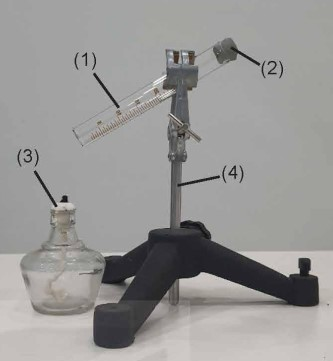
\includegraphics[width=0.3\linewidth]{../figs/VN12-Y24-PH-SYL-003P-5}
\end{center}
\begin{enumerate}[label=\alph*)]
	\item Khi nút chưa bị bật ra, nội năng của không khí trong ống nghiệm không thay đổi.
	\item Nội năng của không khí trong ống nghiệm tăng không chỉ do động năng chuyển động nhiệt của các phân tử khí tăng mà còn do thế năng tương tác giữa chúng tăng.
	\item Nút bấc bị ra là kết quả của áp suất bên trong ống nghiệm giảm đi.
	\item Quá trình nút bấc bật ra ngoài thì khí trong ống đang thực hiện công.
\end{enumerate}
\hideall{
\begin{enumerate}[label=\alph*)]
	\item Sai. Nội năng khí trong ống tăng do nhận nhiệt.
	\item Sai. Thế năng tương tác giữa các phân tử phụ thuộc khoảng cách giữa các phân tử, không phụ thuộc vào nhiệt độ.
	\item Sai. Nút bấc bị ra là kết quả của áp suất bên trong ống nghiệm tăng lên.
	\item Đúng.
\end{enumerate}
}
	
	\item\mkstar{2}\\ 
	Khối khí được chứa trong cylanh, bên trên được nút kín bằng piston cách nhiệt như hình bên dưới. Dùng tay ấn mạnh piston đồng thời nung nóng bên dưới cylanh bằng ngọn lửa đèn cồn.
	\begin{center}
		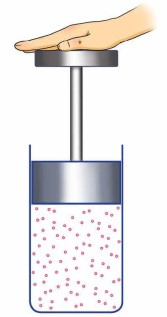
\includegraphics[width=0.15\linewidth]{../figs/VN12-Y24-PH-SYL-003P-3}
	\end{center}
\begin{enumerate}[label=\alph*)]
	\item $A>0$ vì khí nhận công (khí bị nén).
	\item $Q<0$ vì khí bị nung nóng.
	\item Nội năng của khí trong cylanh tăng.
	\item Động năng chuyển động nhiệt của các phân tử khí giảm.
\end{enumerate}
\hideall{
\begin{enumerate}[label=\alph*)]
	\item Đúng.
	\item Sai. Khí nhận nhiệt nên $Q>0$.
	\item Đúng.
	\item Sai. Động năng chuyển động nhiệt của các phân tử khí tăng.
\end{enumerate}
}

\item \mkstar{3}\\
Khi kéo đi kéo lại sợi dây cuốn quanh một ống nhôm đựng nước nút kín, người ta thấy nước trong ống nóng lên rồi sôi, hơi nước đẩy nút bật ra cùng một lớp hơi nước trắng do các hạt nước rất nhỏ tạo thành.
\begin{center}
	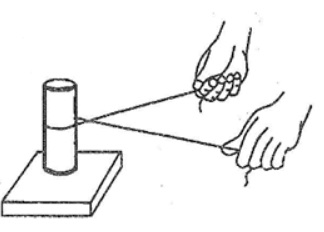
\includegraphics[width=0.3\linewidth]{../figs/VN12-Y24-PH-SYL-003P-4}
\end{center}
\begin{enumerate}[label=\alph*)]
	\item Ống nhôm nóng lên (nội năng ông nhôm tăng) do nhận công.
	\item Có sự truyền nhiệt từ ống nhôm vào nước, làm cho nước nóng lên và hoá hơi.
	\item Quá trình hơi nước làm bật nút là quá trình hơi nước thực hiện công.
	\item Nếu thay nước bằng rượu thì nút sẽ lâu bật ra hơn.
\end{enumerate}
\hideall{
\begin{enumerate}[label=\alph*)]
	\item Đúng.
	\item Đúng.
	\item Đúng.
	\item Sai. Nhiệt độ sôi của rượu thấp hơn nước nên rượu dễ hoá hơi hơn. Quá trình làm nút bật ra sẽ diễn ra nhanh hơn.
\end{enumerate}
}

\item \mkstar{3}\\
Hằng ngày, Mặt Trời truyền về Trái Đất dưới hình thức bức xạ nhiệt một lượng năng lượng khổng lồ, lớn gấp khoảng 20 000 lần tổng năng lượng mà con người sử dụng. 
\begin{center}
	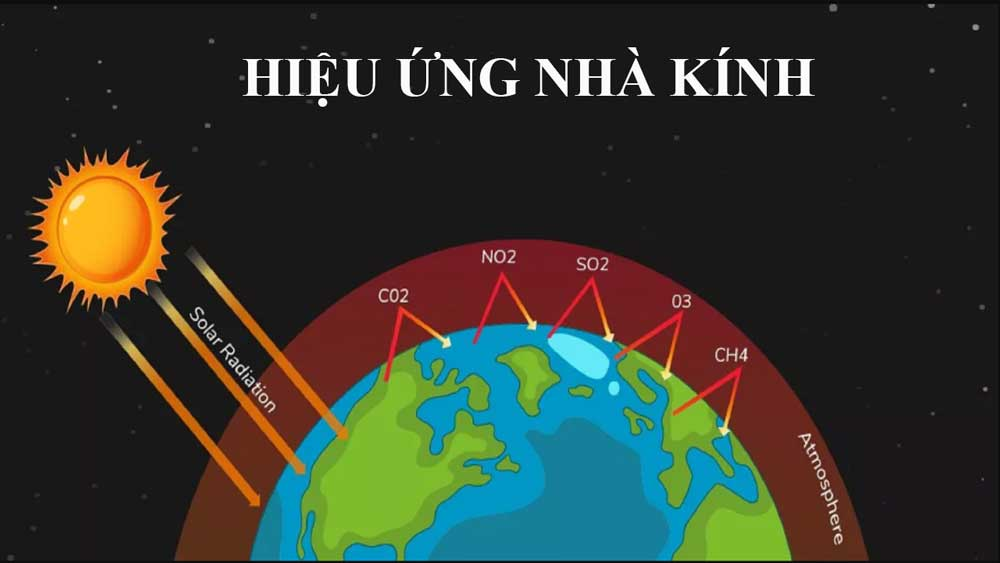
\includegraphics[width=0.45\linewidth]{../figs/VN12-Y24-PH-SYL-003P-6}
\end{center}
Trái Đất hấp thụ một phần năng lượng này, đồng thời phản xạ lại một phần dưới hình thức bức xạ nhiệt của Trái Đất. Bầu khí quyển bao quanh Trái Đất có tác dụng giống như một nhà lợp kính, giữ lại bức xạ nhiệt của Trái Đất làm cho bề mặt của Trái Đất và không khí bao quanh Trái Đất bị nóng lên. Do sự tương tự đó mà hiệu ứng này của bầu khí quyền được gọi là hiệu ứng nhà kính khí quyển, gọi tắt là hiệu ứng nhà kính.\\
Trong khí quyển thì khí carbon dioxide $\left(\ce{CO_2}\right)$ đóng vai trò chủ yếu trong việc gây ra hiệu ứng nhà kính. Hiệu ứng nhà kính vừa có thể có ích vừa có thể có hại. Hiện nay, người ta đang cố gắng làm giảm hiệu ứng nhà kính để ngăn không cho nhiệt độ trên Trái Đất tăng lên quá nhanh, làm đe doạ cuộc sống của con người và các sinh vật khác trên hành tinh này.\\
Nhận định các phát biểu sau đây: 
\begin{enumerate}[label=\alph*)]
	\item Khí nhà kính có vai trò giữ cho nhiệt độ trên Trái Đất không quá lạnh.
	\item Tăng sử dụng động cơ đốt trong có thể làm giảm hiệu ứng nhà kính.
	\item Một phần nguyên nhân của nước biển dâng là do nhiệt độ trên Trái Đất tăng làm cho nước biển bốc hơi nhiều và gây ra mưa nhiều.
	\item Hiệu ứng nhà kính giúp điều hòa nhiệt độ trên Trái Đất, giúp giảm hạn hán và lũ lụt, giảm băng tan trên địa cực và nước biển dâng cao.
\end{enumerate}
\hideall{
\begin{enumerate}[label=\alph*)]
	\item Đúng.
	\item Sai.
	\item Sai.
	\item Sai.
\end{enumerate}
}
\end{enumerate}
\section{Bài tập tự luận}
\begin{enumerate}[label=\bfseries Câu \arabic*:, leftmargin=1.7cm]
	\item \mkstar{2}\\
	Khi đang đóng đinh vào gỗ, mũ đinh có nóng lên nhưng rất ít. Khi đinh đã đóng chắc vào gỗ rồi (không lún thêm được nữa), chỉ cần đóng thêm vài nhát búa là mũ đinh nóng lên rất nhiều. Hãy giải thích?
	\hideall{
	 Khi đang đóng đinh, công thực hiện chuyển thành động năng cho đinh và nội năng cho đinh và búa. Nhưng khi đinh đã được đóng chặt vào gỗ, công thực hiện chỉ chuyển thành nội năng, do đó làm đinh nóng lên nhanh hơn.
}

\item \mkstar{2}\\
Hiện nay, kính cường lực (kính chịu lực rất tốt) thường được sử dụng để làm một phần tường của các toà nhà, trung tâm thương mại, \dots thay thế vật liệu gạch, bê tông. \\
\begin{minipage}{0.6\textwidth}
	Tuy nhiên, vào những ngày nắng nóng, nếu bước vào những căn phòng có tường làm bằng kính cường lực bị đóng kín, ta thường thấy không khí trong phòng nóng hơn so với bên ngoài.
	\begin{enumerate}[label=\alph*)]
		\item Tại sao không khí trong phòng nóng hơn so với không khí ngoài trời?
		\item Hãy đề xuất các biện pháp đơn giản để làm giảm sự tăng nhiệt của không khí trong phòng vào những ngày mùa hè.
	\end{enumerate}
\end{minipage}\hfill
\begin{minipage}{0.4\textwidth}
	\begin{center}
		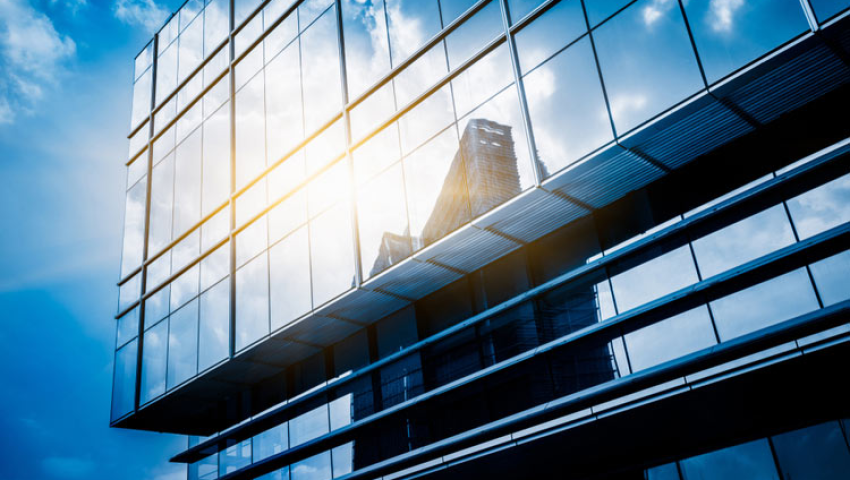
\includegraphics[width=0.7\linewidth]{../figs/VN12-Y24-PH-SYL-003P-1}
	\end{center}
\end{minipage}
\hideall{
\begin{enumerate}[label=\alph*)]
	\item Vào mùa hè, do mặt trời chiếu sáng, không khí trong phòng nhận nhiệt lượng $\left(Q>0\right)$. Do phòng đóng kín nên thể tích khí không đổi, khối khí không sinh công $\left(A=0\right)$. Theo định luật I nhiệt động lực học: $\Delta U=Q+A>0$, nên nội năng của khối khí tăng, làm nhiệt độ không khí trong phòng tăng. Do đó, không khí trong phòng nóng hơn ngoài trời.
	\item Biện pháp đơn giản làm giảm sự tăng nhiệt độ của không khí trong phòng:
	\begin{itemize}
		\item Mở cửa để không khí đối lưu với bên ngoài, từ đó làm nội năng của không khí trong phòng giảm và nhiệt độ phòng giảm xuống.
		\item Lắp rèm cửa: Rèm thường bằng vải dày chuyên dụng, màu sẫm, bề mặt lượn sóng. Khi ánh sáng mặt trời đi qua rèm nó vừa bị phản xạ (do bề mặt, do chất liệu vải), vừa bị hấp thụ (do màu sắc, độ dày của vải). Bên cạnh đó, giữa rèm và mặt kính có có một khoảng ngăn cách, lớp không khí này có khả năng ngăn một phần sự truyền nhiệt từ bên ngoài vào phòng (do không khí dẫn nhiệt kém). Các yếu tố trên làm hạn chế khả năng truyền nhiệt trực tiếp từ Mặt Trời vào sâu bên trong phòng, làm nhiệt độ trong phòng tăng chậm hơn.
		\item Dán tấm phim cách nhiệt: Phim cách nhiệt thường có cấu tạo đặc biệt (từ nhiều lớp polyester và chống ánh sáng tử ngoại), nên khi ánh sáng mặt trời chiếu vào, tấm phim cách nhiệt vừa có tác dụng phản xạ (chủ yếu với ánh sáng hồng ngoại), vừa có tác dụng hấp thụ ánh sáng (chủ yếu với ánh sáng tử ngoại) và truyền qua với các ánh sáng dịu với mắt.
	\end{itemize}
\end{enumerate}
}

\item \mkstar{2}\\
Thực hiện công $\SI{150}{\joule}$ để nén khí trong một cylanh thì khí truyền ra môi trường xung quanh nhiệt lượng $\SI{30}{\joule}$. Xác định độ thay đổi nội năng của khí trong cylanh.
\hideall{
Khí nhận công nên $A>0\Rightarrow A=\SI{150}{\joule}$, khí truyền nhiệt nên $Q<0\Rightarrow Q=\SI{-30}{\joule}$.\\
Độ biến thiên nội năng của khí:
$$\Delta U=Q+A=\SI{120}{\joule}.$$
}

\item \mkstar{3}\\
Giả sử một người đang thực hiện bài vận động vất vả chẳng hạn như nâng tạ hoặc đạp xe. Cơ thể đang thực hiện công và đồng thời nhiệt lượng thoát ra ngoài qua lỗ chân lông vào không khí xung quanh. Theo định luật I nhiệt động lực học, nhiệt độ cơ thể sẽ giảm dần trong quá trình tập luyện. Tuy nhiên, điều đó lại không xảy ra. Như vậy, có phải định luật I nhiệt động lực học không đúng trong trường hợp này phải không? Hãy giải thích.
\hideall{
Trong quá trình vận động cơ thể con người thực hiện công và toả nhiệt ra ngoài môi trường nhưng trong cơ thể người luôn có năng lượng dự trữ để cung cấp năng cho các hoạt động của cơ thể. Năng lượng dự trữ này có được do các quá trình biến đổi chất dinh dưỡng từ thức ăn. Vì vậy, cơ thể luôn được duy trì ở nhiệt độ ổn định và định luật I nhiệt động lực học trong trường hợp này vẫn được nghiệm đúng.
}

\item \mkstar{3}\\
Một quả bóng khối lượng $\SI{200}{\gram}$ rơi từ độ cao $\SI{15}{\meter}$ xuống sân và nảy lên được $\SI{10}{\meter}$. Độ biến thiên nội năng của quả bóng là bao nhiêu? Lấy $g=\SI{10}{\meter/\second^2}$.
\hideall{
Độ biến thiên nội năng của quả bóng:
$$\Delta U=mg\left(h-h'\right)=\SI{10}{\joule}.$$
}


\item \mkstar{3}\\
Một vật khối lượng $\SI{1}{\kilogram}$ trượt không vận tốc đầu từ đỉnh xuống chân một mặt phẳng dài $\SI{21}{\meter}$, nghiêng $\SI{30}{\degree}$ so với mặt nằm ngang. Tốc độ của vật ở chân mặt phẳng nghiêng là $\SI{4.1}{\meter/\second}$. Tính công của lực ma sát và độ biến thiên nội năng của vật trong quá trình chuyển động trên. Lấy $g=\SI{9.8}{\meter/\second^2}$. Bỏ qua sự trao đổi nhiệt với mặt phẳng nghiêng.
\hideall{
Công của lực ma sát:
$$A_\text{ms}=W_\text{s}-W_\text{t}=mgh_\text{s}+\dfrac{1}{2}mv^2_\text{s}-mgh_\text{t}-\dfrac{1}{2}mv^2_\text{t}=\dfrac{1}{2}mv^2_\text{s}-mg\ell\sin\SI{30}{\degree}\approx\SI{-94.5}{\joule}.$$
Độ biến thiên nội năng của vật trong quá trình chuyển động bằng công của lực ma sát:
$$\Delta U=\SI{94.5}{\joule}.$$
}
\end{enumerate}






